\section{Обзор предметной области}
\label{section:Theory}
В данном разделе будет произведён обзор предметной области задачи, решаемой в рамках данной дипломной работы; рассмотрены вопросы о назначении, областях применения и принципах работы акустической камеры и приведены теоретические сведения об её отдельных элементах, а также некоторые критерии выбора их параметров. 

% **************************************************
\subsection{Акустическая камера}
Акустическая камера (англ. \foreignlanguage{english}{acoustic camera})~--- это устройство позволяющее обнаруживать источники звука и определять их характеристики~\cite{Wiki_AcousticCamera}. Она состоит из набора микрофонов, называемых микрофонной решёткой. Эти датчики одновременно улавливают звуковые волны от источников звука. Данные полученные с микрофонов обрабатываются специальным образом, что позволяет определить местоположения источников. Для наглядности звуковой картины, её совмещают с видео-изображением с видео-камеры, которую обычно располагают в центре микрофонной решётки.

\begin{figure}[ht]
	\centering
	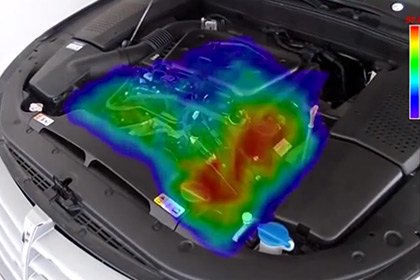
\includegraphics[scale=1]{AcWorkExample.jpg}  
	\caption{Пример работы коммерческого образца акустической камеры}
	\label{fig:AcWorkExample}
\end{figure}

Результат работы акустической камеры обычно выглядит так, как показано на рисунке~\ref{fig:AcWorkExample}

\subsubsection{Применение. }
Существует множество различных применений для акустической камеры, главным из которых является обнаружение источников шума, для их последующего устранения. Камера помогает улучшать шумовые характеристики различных транспортных средств (автомобили, поезда, самолёты) и сооружений (например, турбин). 

С помощью данного устройства, можно не только оценивать характеристики шума излучаемого объектами во внешнюю среду, но улучшать акустический комфорт помещений и кабин транспортных средств.

Поиск причин выхода из строя различных механизмов также можно производить с использованием акустической камеры. Для этого необходимо проанализировать звуковые картины исправного и неисправного механизмов.

Не исключено и военное применение данного устройства. Например, наблюдая за звуковой картиной местности, возможно обнаружить направление, с которого противник ведёт огонь.

В случае разработки дешёвой и компактной акустической камеры не исключено её использование в качестве необычного гаджета.

\subsubsection{Структура и принцип работы. }
Для того, чтобы понять, как работает акустическая камера, взглянем на её функциональную схему, изображённую на рисунке~\ref{fig:AcousticCameraDiagram}. Из данной схемы видно, что вся система состоит из 4 функциональных блоков:
\begin{itemize}
	\item Микрофонная решётка. Данное устройство играет роль датчика, благодаря которому можно определять положение источников звука в пространстве. Более подробная информация о микрофонных решётках приведена в разделе~\ref{section:MicrophoneArrays};
	\item Видеокамера. Это устройство производит съёмку анализируемого объекта и некоторого пространства вокруг него, чтобы построить более понятное человеку изображение. Чаще всего видеокамеру располагают в центре микрофонной решётки, для облегчения задачи совмещения видеоизображения и данных полученных с микрофонной решётки;
	\item Вычислительный модуль служит для анализа данных приходящих с микрофонной решётки и совмещения результатов этого анализа с видеоизображением. Такой анализ можно произвести при помощи пространственной фильтрации, подробнее о которой рассказано в разделе~\ref{section:SpatialFiltering}. Также данный модуль может использоваться для расчётов звукового давления и перевода его в необходимые единицы измерения, если это необходимо;
	\item Устройство вывода необходимо для отображения полученных вычислительным модулем данных. В его качестве можно использовать обычный жидкокристаллический монитор.
\end{itemize}

\begin{figure}[ht]
	\centering
	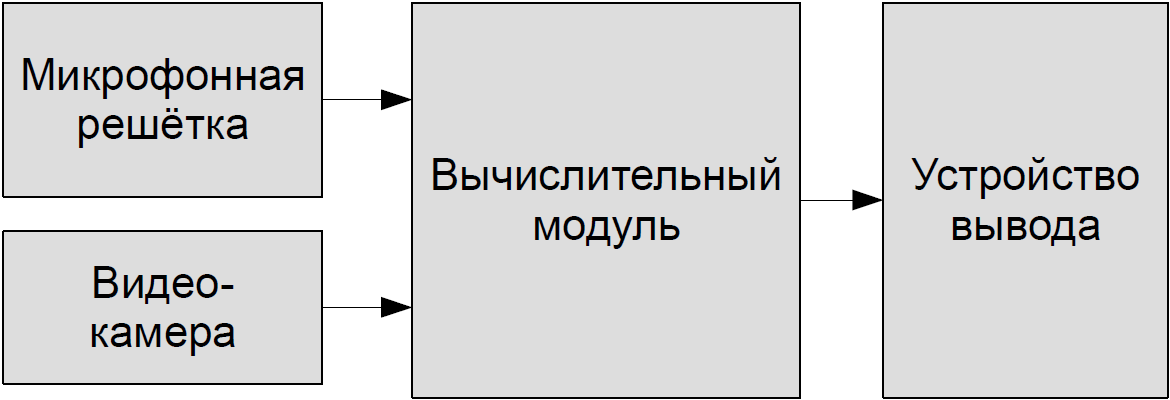
\includegraphics[scale=0.5]{AcousticCameraDiagram.png}  
	\caption{Функциональная схема акустической камеры}
	\label{fig:AcousticCameraDiagram}
\end{figure}

% **************************************************
\subsection{Микрофонные решётки}
\label{section:MicrophoneArrays}
Микрофонная решётка (массив микрофонов)~--- система микрофонов, расположенных определённым образом друг относительно друга. Чаще всего используемые в этой системе микрофоны являются всенаправленными. При дальнейшей обработке данных с такой решётки возможно сформировать заданную диаграмму направленности всей системы без изменения её физических параметров.

\subsubsection{Одномерные решётки. }
Самым простым типом микрофонных решёток является линейная решётка, расположение микрофонов в которой показано на рисунке~\ref{fig:LinearMicArray}. Как видно из рисунка эта решётка является одномерной, следовательно по данным полученным с такой решётки возможно построить лишь одномерную звуковую картину. Однако, несмотря на невозможность построения полноценной двумерной картины, простота конструкции и обработки получаемых с решётки данных, делают такую конфигурацию микрофонов весьма привлекательной для использования в прототипе.

\begin{figure}[ht]
	\centering
	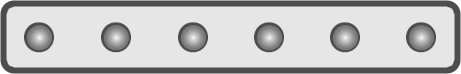
\includegraphics[scale=1]{MicArrayConfigLinear.png}  
	\caption{Линейная микрофонная решётка}
	\label{fig:LinearMicArray}
\end{figure}

\subsubsection{Двумерные решётки. }
Для того, чтобы построить двумерную карту источников звука, необходимо использовать двуменрные микрофонные решётки.

Двумерные решётки, данные с которых обрабатываются с помощью так называемого бимформинга (см. раздел ~\ref{section:Beamforming}), чаще всего имеют круглую форму. Конфигурации, согласно которым располагают элементы таких решёток обычно бывают следующих типов~\cite[с.~5]{NI_AcousticBeamforming}:
\begin{itemize}
	\item Круговая;
	\item Спиральная;
	\item Случайная.
\end{itemize}

Круговая конфигурация подходит для систем, в которых не известно точное расстояние до источника звука, но при этом ей присущ узкий динамический диапазон. Спиральная конфигурация, даёт лучшие результаты, однако, наилучшие параметры микрофонная решётка имеет при случайном расположении сенсоров. Такое расположение микрофонов позволяет достичь наилучшего динамического диапазона~\cite[с.~5]{NI_AcousticBeamforming}. Примеры описанных конфигураций приведены на рисунке~\ref{fig:MicArrayConfigs}

\begin{figure}[ht]
\centering
  \begin{subfigure}[b]{0.45\textwidth} 
    \centering
    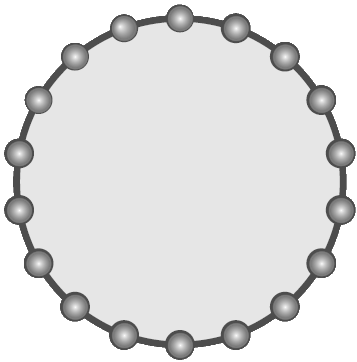
\includegraphics[scale=0.6]{MicArrayConfigRing.png}  
    \caption{}
  \end{subfigure}
  \begin{subfigure}[b]{0.45\textwidth} 
    \centering
    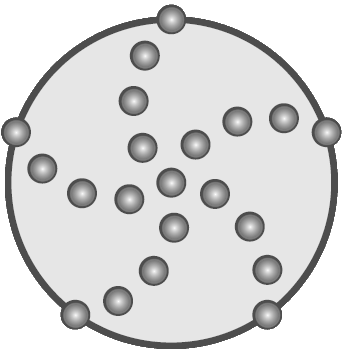
\includegraphics[scale=0.6]{MicArrayConfigSpiral.png}  
    \caption{}
  \end{subfigure}
  \begin{subfigure}[b]{0.45\textwidth} 
    \centering
    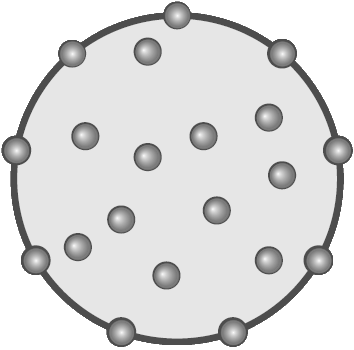
\includegraphics[scale=0.6]{MicArrayConfigRandom.png}  
    \caption{}
  \end{subfigure}
  \caption{ Конфигурации микрофонных решёток:
			а "--- круговая;
            б "--- спиральная;
			в "--- случайная.}
  \label{fig:MicArrayConfigs}
\end{figure}

% **************************************************
\subsection{Пространственная фильтрация}
\label{section:SpatialFiltering}
Пространственная фильтрация~--- процесс выделения сигналов приходящих с желательных направлений и подавления сигналов приходящих с нежелательных направлений из всех сигналов регистрируемых датчиком. 

\begin{figure}[ht]
	\centering
	\includegraphics[scale=0.5]{Screening.png}  
	\caption{Экранирование датчика. Чёрной сплошной стрелкой показан желательный сигнал, а серыми пунктирными нежелательные сигналы.}
	\label{fig:Screening}
\end{figure}

Самым простым способом реализации пространственной фильтрации является экранирование (см. рисунок~\ref{fig:Screening}), при котором сигналы с нежелательных направлений механически изолируются от датчика. Но к сожалению, такой подход имеет существенный недостаток, а именно невозможность изменять диаграмму направленности датчика без изменения физических параметров экрана.

Однако, в последнее время появились и более совершенные подходы к пространственной фильтрации.

\subsection{Бимформинг}
\label{section:Beamforming}
В связи с бурным развитием вычислительной техники и совершенствованием алгоритмов цифровой обработки сигналов, появился новый более гибкий метод пространственной фильтрации, с помощью устройства, которое называется <<бимформер>>. Данный термин является калькой с английского \foreignlanguage{english}{beamformer}, что при дословном переводе означает лучеформирователь.

Бимформер~--- это вычислительное устройство, используемое совместно с массивом датчиков, для выполнения пространственной фильтрации сигналов. Массив датчиков собирает пространственные выборки амплитуды распространяющейся волны, которые обрабатываются бимформером. Главной задачей является оценка направления с которого пришёл желаемый сигнал в присутствии шумов и прочих сигналов интерферирующих с желаемым. Бимформер выполняет пространственную фильтрацию, чтобы разделить сигналы имеющие одинаковые спектральные составляющие, но приходящие с разных направлений~\cite{IEEE_Beamforming}.

Процесс фильтрации с использованием бимформера называют бимформингом.

Выделяют три основных типа бимформинга~\cite{Wiki_SensorArray}:
\begin{itemize}
	\item \dands{} бимформинг
	\item Спектральный бимформинг
	\item Параметрический бимформинг
\end{itemize}
Наиболее простым в реализации, но имеющий худшие характеристики по сравнению с остальными типами является \dands{} бимформинг.

\subsubsection{\dands{} бимформинг. }
\label{section:DelayAndSumBeamforming}
Термин \dands{} при дословном переводе означает задержи и сложи. Принцип работы бимформера, построенного по такой схеме, продемонстрирован на рисунке~\ref{fig:DelayAndSumDiagram}

\begin{figure}[ht]
	\centering
	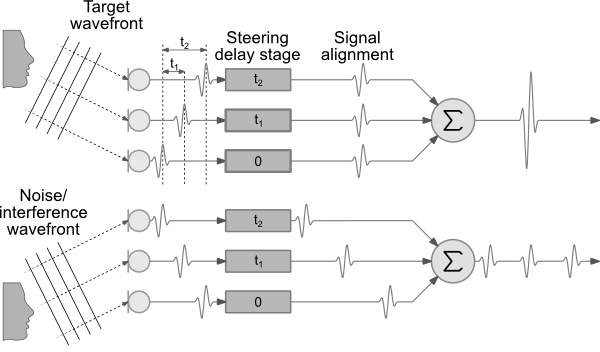
\includegraphics[scale=0.7]{DelayAndSumDiagram.png}  
	\caption{Схема работы \dands{} бимформера}
	\label{fig:DelayAndSumDiagram}
\end{figure}

Данная система состоит из трёх микрофонов, трёх элементов задержки с задержками $0$, $t_1$, $t_2$ и сумматора. Из рисунка можно заметить, что от направления на источник звука зависит разница времени прихода звуковой волны на микрофоны. При фиксированных значениях $t_1$ и $t_2$ звуковой сигнал, приходящий с одного из направлений, будет равен сумме сигналов с трёх микрофонов. Это хорошо видно в верхней части рисунка. В другой части рисунка, сигнал приходит с другого направления, но из-за другой разницы фаз, результирующий сигнал равен сигналу с каждого микрофона в отдельности, а значит, его амплитуда в 3 раза меньше. Таким образом, варьируя значения $t_1$ и $t_2$, можно менять направление, в котором решётка из трёх микрофонов будет наиболее чувствительна.

Применив двумерную решётку и просканировав множество направлений можно построить карту расположения источников звука.

% **************************************************
\subsection{Плотностно-импульсная модуляция}
\label{section:pdm}
Плотностно-импульсная модуляция (\foreignlanguage{english}{pulse-density modulation, PDM}, cигма-дельта модуляция)~--- Способ модуляции используемый для представления аналогового сигнала в цифровой форме. В сигнале закодированном таким образом определённые значения амплитуд не кодируются с помощью слов состоящих из импульсов, имеющих различный вес, как это делается в импульсно-кодовой модуляции. Вместо этого используется относительная плотность импульсов, которая соответствует амплитуде исходного аналогового сигнала~\cite{Wiki_PDM}.

Для того, чтобы понять принцип работы данного вида модуляции, рассмотрим сначала принцип работы дельта-модуляции.

\subsubsection{Дельта-модуляция. }
Рассмотрим блок-схему дельта-модулятора, изображённую на рисунке~\ref{fig:DeltaModulation}.

\begin{figure}[ht]
	\centering
	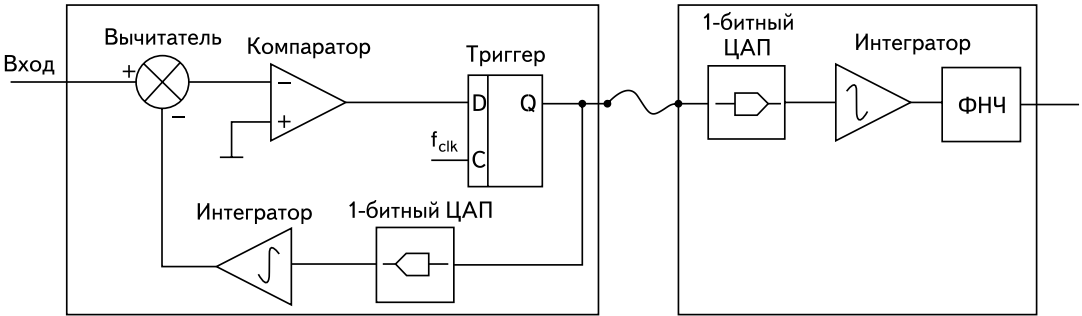
\includegraphics[scale=0.55]{DeltaModulation.png}  
	\caption{Блок-схема дельта-модулятора: ФНЧ~--- фильтр низких частот}
	\label{fig:DeltaModulation}
\end{figure}

Принцип его действия можно описать следующим образом: на основании некоторого набора предыдущих выборок сигнала делается предположение о последующей. Затем предполагаемое значение сравнивается с фактическим и выносится решение о знаке их различия, что и является выходным сигналом~\cite{KitE_DeltaSigma}.

Напряжение входного сигнала подаётся на вычитатель, где из него вычитается аппроксимирующее напряжение, созданное на основании предыдущих значений сигнала. Далее разность поступает на стробируемый компаратор, где сравнивается с нулевым уровнем. Таким образом, логическая единица на выходе компаратора означает, что эта разность положительна или что входной сигнал больше предполагаемого (аппроксимирующего), а логический ноль, соответственно, означает, что входной сигнал меньше аппроксимирующего. Далее последовательность нулей и единиц поступает на однобитный местный ЦАП, который обычно представляет из себя преобразователь уровней одно-полярного напряжения (лог. «0» и лог. «1») в двухполярное ($\pm{}U_{\text{пит}}$). С выхода ЦАП сигнал поступает на вход интегратора, на выходе которого формируется аппроксимирующее напряжение, с заданной точностью повторяющее входное. Точность определяется частотой стробирования компаратора и шагом приращения напряжения в интеграторе. Схема приёмной части состоит из однобитного ЦАП, интегратора и ФНЧ~\cite{KitE_DeltaSigma}.

Эта схема имеет ряд существенных недостатков, которые препятствовали ее применению в аппаратуре аналогово-цифрового преобразования. Попытки её модернизации привели к переходу от дельта-модуляции к дельта-сигма модуляции~\cite{KitE_DeltaSigma}.

\subsubsection{Дельта-сигма модуляция. }
Этот тип модуляции обладает всеми достоинствами дельта-модуляции и в то же время лишён многих её недостатков. Для того чтобы разобраться в его структуре и понять, как был выполнен переход от схемы дельта-модулятора к схеме дельта-сигма модулятора (ДСМ), можно рассуждать следующим образом. Как известно, дельта-модулятор пригоден для работы только с хорошо коррелированными сигналами, поэтому для повышения коррелированности входного сигнала его можно пропустить через интегратор, а на приёмной стороне выходной преобразованный сигнал пропустить, соответственно, через дифференциатор~\cite{KitE_DeltaSigma} (см. рисунок~\ref{fig:DeltaToDeltaSigma}).

\begin{figure}[ht]
	\centering
	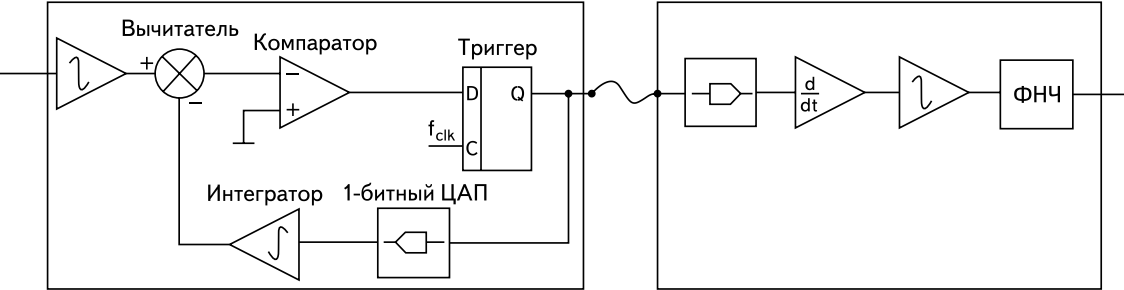
\includegraphics[scale=0.55]{DeltaToDeltaSigma.png}  
	\caption{Переход от дельта-модулятора к дельта-сигма модулятору}
	\label{fig:DeltaToDeltaSigma}
\end{figure}

Поскольку разность интегралов равна интегралу разности, то два интегратора на входах вычитателя можно заменить одним на его выходе. Что касается дифференциатора на приёмной стороне, то он вместе с приёмным интегратором может быть исключён. Таким образом, схема ДСМ, изображённая на рисунке~\ref{fig:DeltaSigmaModulation}, отличается от дельта-модулятора положением интегратора на передающей стороне и его отсутствием на приёмной. Такое незначительное изменение в схеме значительно улучшило её характеристики и, в частности, позволило достичь отношения сигнал/шум -120 дБ~\cite{KitE_DeltaSigma}.

\begin{figure}[ht]
	\centering
	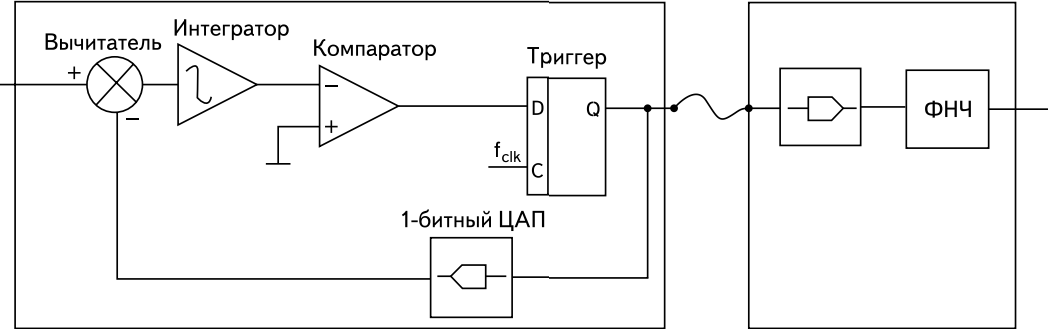
\includegraphics[scale=0.55]{DeltaSigmaModulation.png}  
	\caption{Схема дельта-сигма модулятора}
	\label{fig:DeltaSigmaModulation}
\end{figure}

Рассмотрим работу схемы ДСМ. Когда образуется высококоррелированный сигнал, то коррелированными оказываются не только его отсчёты, но и ошибки при каждом квантовании. Следовательно, их легко предсказать и вычесть из сигнала, отправляемого на устройство квантования, прежде чем произойдёт квантование. Хорошей оценкой текущей ошибки в таком случае выступает предшествующая ошибка. Предшествующая ошибка, образованная как разность между входом и выходом устройства квантования, помещается в схему задержки (триггер). Таким образом, в контуре обратной связи циркулирует сигнал ошибки~\cite{KitE_DeltaSigma}.

Выходной сигнал ДСМ представляет собой однобитный поток импульсов. Рассмотрим его в терминах теории вероятности. Так, вероятность появления в потоке логической единицы $P(1)$ и вероятность появления логического нуля $P(0)$ связаны следующим выражением: $P(0)+P(1) = 1$. Более того, если на вход модулятора подаётся некий сигнал (ограниченный в динамическом диапазоне 0~--~1), то вероятность $P(1)=x$, а $P(0)=(1-x)$. Иными словами, чем плотнее представлены импульсы определённой полярности в потоке, тем выше уровень сигнала в этот момент. Нулевой уровень сигнала кодируется одинаковой плотностью положительных и отрицательных импульсов. Импульсные последовательности при кодировании синусоидального напряжения представлены на рисунке~\ref{fig:DeltaSigmaOscillogram}. Видно, что плотность положительных и отрицательных импульсов одинакова в точках, близких к 0, плотность отрицательных импульсов максимальна в точке $-1$, и плотность положительных импульсов максимальна в точке $+1$~\cite{KitE_DeltaSigma}.

\begin{figure}[ht]
	\centering
	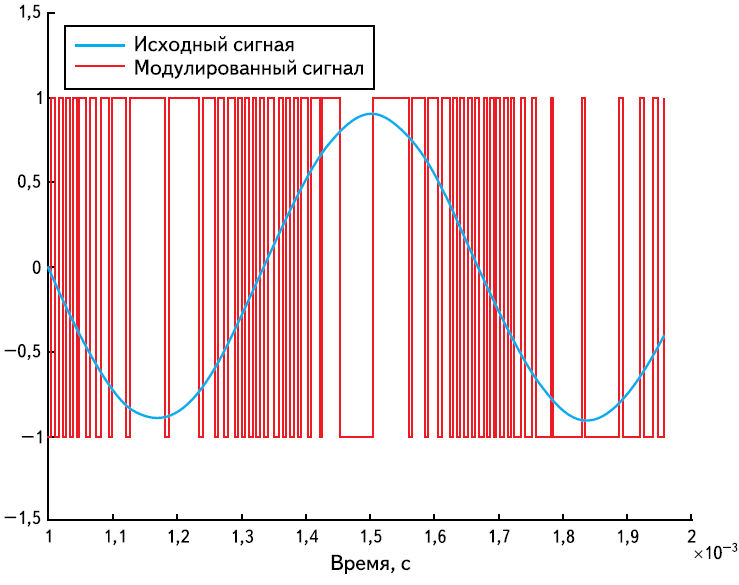
\includegraphics[scale=0.8]{DeltaSigmaOscillogram.png}  
	\caption{Осциллограмма выходного сигнала дельта-сигма модулятора}
	\label{fig:DeltaSigmaOscillogram}
\end{figure}

Такие особенности позволяют кодировать в формате дельта-сигма модуляции сигналы с частотой от 0 до 100 кГц. В частности, прямоугольное аналоговое напряжение и уровни постоянного напряжения, последнее актуально при применении дельта-сигма модуляции в датчиках медленно меняющихся сигналов~\cite{KitE_DeltaSigma}.

\begin{figure}[ht]
\centering
  \begin{subfigure}[b]{0.45\textwidth} 
    \centering
    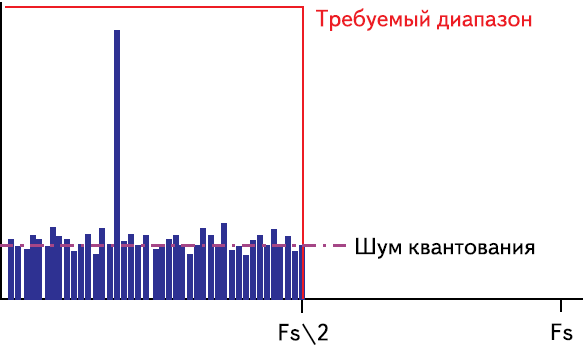
\includegraphics[scale=0.45]{OutputSpectrumA.png}  
    \caption{}
  \end{subfigure}
  \begin{subfigure}[b]{0.45\textwidth} 
    \centering
    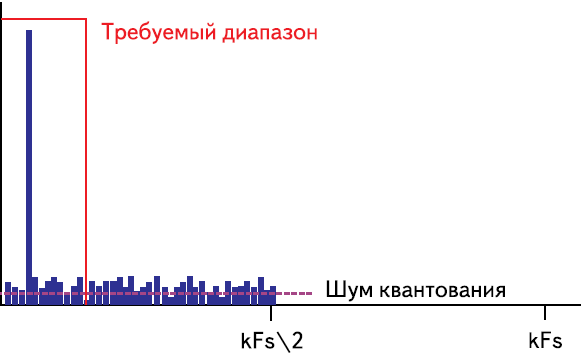
\includegraphics[scale=0.45]{OutputSpectrumB.png}  
    \caption{}
  \end{subfigure}
  \begin{subfigure}[b]{0.45\textwidth} 
    \centering
    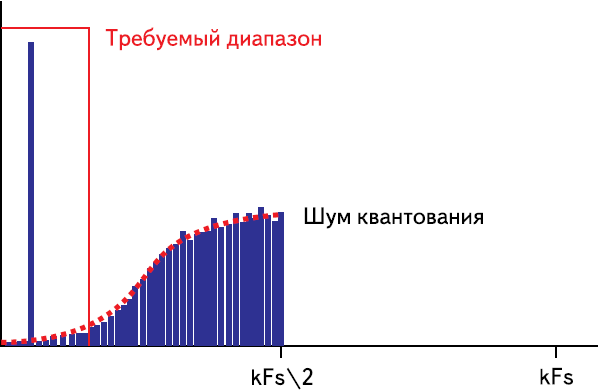
\includegraphics[scale=0.45]{OutputSpectrumC.png}  
    \caption{}
  \end{subfigure}
  \caption{ Спектры выходного сигнала:
			а "--- при обычных условиях;
            б "--- при оверсемплинге;
			в "--- при использовании нойзшейпинга.}
  \label{fig:OutputSpectrum}
\end{figure}

\subsubsection{Шумы. }
Исследование шумов в ДСМ заслуживает отдельного рассмотрения. Ведь методы достижения отношения сигнал/шум -120 дБ при разрядности 1 бит представляют известный интерес. В 1954 году С. Катлер из той же лаборатории Александра Бэлла предложил концепцию передискретизации и формирования спектра шума. Как известно, каждый дополнительный бит при преобразовании аналогового сигнала в цифровой добавляет 6 дБ к отношению сигнал/шум (рисунок~\ref{fig:OutputSpectrum}a). Одним из основополагающих принципов дельта-модуляции является превышение частоты Котельникова в К раз. При такой передискретизации эффективная разрядность, а соответственно, и отношение сигнал/шум, увеличивается согласно формуле $K=2^N$, где $K$~--- коэффициент передискретизации, а $N$~--- количество дополнительных битов. Обычно применяется $K=64$, и в этом случае эффективная разрядность будет 7 бит, а отношение сигнал/шум будет равно 42 дБ (рисунок~\ref{fig:OutputSpectrum}б). Однако передискретизация сама по себе не является эффективным средством. Дальнейшее подавление шума производится благодаря самой структуре дельта-сигма модулятора. В иностранной литературе часто применяется термин <<нойзшейпинг>> (англ. \foreignlanguage{english}{noise shaping}), что означает формирование спектра шума. Чтобы понять, как именно происходит формирование, используем линеаризованную дискретную модель системы, в которой входной сигнал представлен последовательностью $x(n)$, выходной сигнал $y(x)$ и шум квантования, вносимый компаратором и триггером,~--- $e(n)$, что изображено на рисунке~\ref{fig:DeltaSigmaLinearModel}~\cite{KitE_DeltaSigma}.

\begin{figure}[ht]
	\centering
	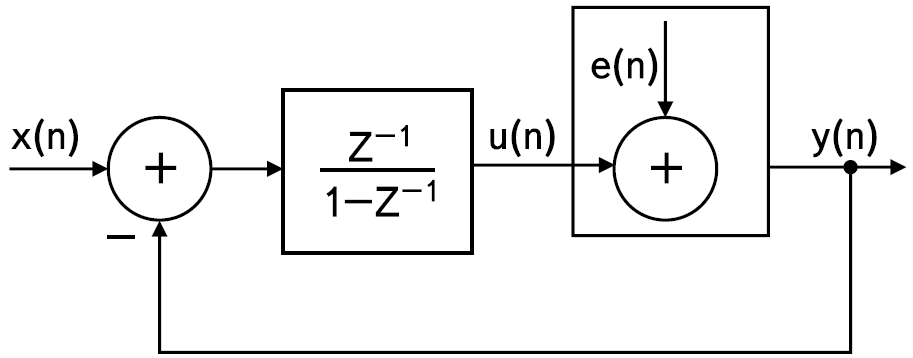
\includegraphics[scale=0.6]{DeltaSigmaLinearModel.png}  
	\caption{Осциллограмма выходного сигнала дельта-сигма модулятора}
	\label{fig:DeltaSigmaLinearModel}
\end{figure}

Рассмотрим Z-преобразование этой системы дельта-сигма модулятора:

\begin{gather}
	Y(z)=\frac{X(z)-Y(z)}{z\left(1-\frac{1}{z}\right)}+E(z), \\
	Y(z)=\frac{X(z)}{z}+\left(1-\frac{1}{z}\right)E(z).
\end{gather}

Видно, что полезный сигнал $X(z)$ проходит эту цепь без изменений, с задержкой на 1 такт, в то время как для шума возникает препятствие в виде ФНЧ. Таким образом, осуществляется формирование спектра шума в дельта-сигма модуляторе. Интегратор в данном случае выступает в качестве ФНЧ для шумовой составляющей сигнала. Энергия шума сосредотачивается в области верхних частот, и большая ее часть может быть отфильтрована выходным ФНЧ (рисунок~\ref{fig:OutputSpectrum}в). Таким образом, в выходном сигнале после демодулирования дельта-сигма последовательности наблюдается намного более низкий уровень шума, чем можно было бы предполагать. Следующим шагом по улучшению параметров по шумам является повышение порядка модулятора. Следует особо отметить, что дельта-сигма АЦП с высочайшей (24 бита) эффективной разрядностью можно построить, всего лишь используя интегратор и стробируемый компаратор~\cite{KitE_DeltaSigma}.

\subsubsection{Информационные параметры. }
Еще одним важным на сегодня параметром сигнала является его информационная ёмкость. Здесь следует отметить, что сигнал в формате дельта-сигма модуляции не требует кадровой синхронизации, а значит, считывать его можно в любой момент времени в записи или в канале передачи. В этом его сходство с аналоговым сигналом. Ещё одно важное его отличие~--- это факт одинаковой информационной ёмкости каждого бита в потоке, что повышает помехоустойчивость сигнала в формате дельта-сигма модуляции~\cite{KitE_DeltaSigma}.

Оценим теперь информационные параметры сигнала. В качестве требуемого диапазона возьмем порог слышимости, принятый в различных стандартах звукозаписи,~--- 22 кГц. Частота Котельникова в ИКМ для такого диапазона, следовательно, будет равняться 44 кГц. Оверсэмплинг в формате дельта-сигма модуляции (например, SACD фирмы Sony) предполагает 64-кратное увеличение частоты Котельникова. Таким образом, получается, что частота дискретизации в формате дельта-сигма модуляции с овер-сэмплингом будет равна 2,82 МГц для передачи диапазона от 0 до 22 кГц. Учитывая, что передача цифровых сигналов в обоих форматах ведётся в последовательном режиме, оценим количество бит в секунду. При последовательной передаче в формате ИКМ 44 кГц/16 бит поток равен 705 кБод, в формате дельта-модуляции~--- 2,8 мБод. Однако качество сигнала в формате дельта-модуляции 2,8 МГц приближается к качеству сигнала в формате ИКМ~--- 192 кГц/24 бита, поток которого составляет уже 4,8 мБод. Также следует учесть, что, в отличие от дельта-сигма модуляции, при передаче ИКМ-сигналов требуется жёсткая кадровая синхронизация~\cite{KitE_DeltaSigma}.

% **************************************************
\subsection{Общие сведения о цифровых фильтрах}
\label{section:DigitalFilters}
Цифровой фильтр~--- в электронике любой фильтр, обрабатывающий цифровой сигнал с целью выделения и/или подавления определённых частот этого сигнала. В отличие от цифрового, аналоговый фильтр имеет дело с аналоговым сигналом, его свойства недискретны, соответственно передаточная функция зависит от внутренних свойств составляющих его элементов~\cite{Wiki_DigitalFilter}.

\subsubsection{Применение. }
Цифровые фильтры на сегодняшний день применяются практически везде, где требуется обработка сигналов, в частности в спектральном анализе, обработке изображений, обработке видео, обработке речи и звука и многих других приложениях~\cite{Wiki_DigitalFilter}.

\subsubsection{Характеристика цифровых фильтров. }
Линейный стационарный цифровой фильтр характеризуется передаточной функцией. Передаточная функция может описать, как фильтр будет реагировать на входной сигнал. Таким образом, проектирование фильтра состоит из постановки задачи (например, фильтр восьмого порядка, фильтр нижних частот с конкретной частотой среза), а затем производится расчёт передаточной функции, которая определяет характеристики фильтра~\cite{Wiki_DigitalFilter}.

Передаточная функция фильтра имеет вид:
\begin{equation}
	H(z)=\frac{B(z)}{A(z)}=\frac{b_0+b_1z^{-1}+b_2z^{-2}+...+b_Nz^{-N}}{1+a_1z^{-1}+a_2z^{-2}+...+a_Mz^{-M}},
\end{equation}
\begin{explanation}
	где & порядок фильтра & большее $N$ или $M$.
\end{explanation}
В данном случае это формула БИХ-фильтра. Если знаменатель равен единице, то получаем формулу КИХ-фильтра (без обратной связи)~\cite{Wiki_DigitalFilter}.

\subsubsection{Преимущества. }
Преимуществами цифровых фильтров перед аналоговыми являются~\cite{Wiki_DigitalFilter}:
\begin{itemize}
	\item Высокая точность (точность аналоговых фильтров ограничена допусками на элементы);
	\item Стабильность (в отличие от аналогового фильтра передаточная функция не зависит от дрейфа характеристик элементов);
	\item Гибкость настройки, лёгкость изменения;
	\item Компактность~--- аналоговый фильтр на очень низкую частоту (доли герца, например) потребовал бы чрезвычайно громоздких конденсаторов или индуктивностей.
\end{itemize}

\subsubsection{Недостатки. }
Недостатками цифровых фильтров по сравнению с аналоговыми являются~\cite{Wiki_DigitalFilter}:
\begin{itemize}
	\item Трудность работы с высокочастотными сигналами. Полоса частот ограничена частотой Найквиста, равной половине частоты дискретизации сигнала. Поэтому для высокочастотных сигналов применяют аналоговые фильтры, либо, если на высоких частотах нет полезного сигнала, сначала подавляют высокочастотные составляющие с помощью аналогового фильтра, затем обрабатывают сигнал цифровым фильтром;
	\item Трудность работы в реальном времени — вычисления должны быть завершены в течение периода дискретизации;
	\item Для большой точности и высокой скорости обработки сигналов требуется не только мощный процессор, но и дополнительное, возможно дорогостоящее, аппаратное обеспечение в виде высокоточных и быстрых ЦАП и АЦП.
\end{itemize}

\subsubsection{Виды. }
Цифровые фильтры подразделяют на два основных класса:
\begin{itemize}
	\item КИХ-фильтры
	\item БИХ-фильтры
\end{itemize}

% **************************************************
\subsection{Фильтр с бесконечной импульсной характеристикой}
\label{section:IIR}
Фильтр с бесконечной импульсной характеристикой (рекурсивный фильтр, БИХ-фильтр) или IIR-фильтр (IIR сокр. от англ. \foreignlanguage{english}{infinite impulse response}~--- бесконечная импульсная характеристика)~--- линейный электронный фильтр, использующий один или более своих выходов в качестве входа, то есть образует обратную связь. Основным свойством таких фильтров является то, что их импульсная переходная характеристика имеет бесконечную длину во временной области, а передаточная функция имеет дробно-рациональный вид. Такие фильтры могут быть как аналоговыми, так и цифровыми~\cite{Wiki_IIR}.

Примерами БИХ-фильтров являются~\cite{Wiki_IIR}:
\begin{itemize}
	\item Фильтр Чебышёва;
	\item Фильтр Баттерворта;
	\item Фильтр Калмана;
	\item Фильтр Бесселя.
\end{itemize}

\subsubsection{Динамические характеристики. }
Разностное уравнение, описывающее дискретный БИХ-фильтр, устанавливает связь между входным и выходным сигналами во временной области:
\begin{eqnarray}
	y(n) = b_{0} x(n) + b_{1} x(n-1) + \cdots + b_{P} x(n-P) - \nonumber \\
	- a_{1} y(n-1) - a_{2} y(n-2) - \cdots - a_{Q} y(n-Q),
\end{eqnarray}
\begin{explanation}
	где &$P$& порядок входного сигнала; \\
	&$b_{i}$& коэффициенты входного сигнала; \\
	&$Q$& порядок обратной связи; \\
	&$a_{i}$& коэффициенты обратной связи; \\
	&$x(n)$& входной сигнал; \\
	&$y(n)$& выходной сигнал; \\
\end{explanation}
Более компактная запись разностного уравнения:
\begin{equation}
	y(n) = \sum_{i=0}^P b_{i}x(n-i) - \sum_{k=1}^Q a_{k} y(n-k).
\end{equation}
Для того, чтобы найти ядро фильтра, положим:
\begin{equation}
	x(n) = \delta(n),
\end{equation}
\begin{explanation}
	где &$\delta(n)$& дельта-функция.
\end{explanation}
Тогда импульсная переходная функция (ядро фильтра) записывается как:
\begin{equation}
	h(n)=\sum_{i=0}^P b_{i}\delta(n-i) - \sum_{k=1}^Q a_{k} h(n-k).
\end{equation}
Z-преобразование импульсной переходной функции даёт передаточную функцию БИХ-фильтра~\cite{Wiki_IIR}:
\begin{equation}
	H(z)= \frac{\sum_{i=0}^P b_{i} z^{-i}}{1+\sum_{k=1}^Q a_{k} z^{-k}}.
\end{equation}

\subsubsection{Устойчивость. }
Об устойчивости фильтра с бесконечной импульсной характеристикой судят по его передаточной функции. Для дискретного фильтра необходимо и достаточно, чтобы все полюса его передаточной функции по модулю были меньше единицы (т. е. лежали внутри единичного круга на z-плоскости). Все критерии устойчивости, применимые в теории линейных стационарных систем, например критерий устойчивости Найквиста или критерий устойчивости Рауса применимы и в случае БИХ-фильтров~\cite{Wiki_IIR}.

В отличие от КИХ-фильтров, БИХ-фильтры не всегда являются устойчивыми~\cite{Wiki_IIR}.

\subsubsection{Реализация БИХ фильтра. }
Если рассматривается передаточная функция вида:
\begin{equation}
	H(z) = \frac{Y(z)}{X(z)} = \frac{\sum_ {k=0}^{M} b_{k} z ^{-k} } { 1 + \sum_ {k=1}^{N} a_{k} z ^{-k}} = \frac{B(z)}{A(z)}, 
\end{equation}
то соотношение между входом и выходом такой системы должно удовлетворять разностному уравнению:
\begin{equation}
	y(n) = -\sum_ {k=1}^N a(k)y(n - k) + \sum_ {k=0}^M b(k)x(n - k).
\end{equation}
Это уравнение может быть записано непосредственно из выражения для передаточной функции, таким образом форму построения цепи, соответствующей этому уравнению, называют прямой формой I~\cite{Wiki_IIR}.

При построении БИХ фильтра для простоты можно принять, что $M=N$. БИХ фильтры могут быть реализованы с использованием трёх элементов или основных операций: умножитель, сумматор и блок задержки. Этих элементов достаточно для всех возможных цифровых фильтров. вариант, показанный на рисунке~\ref{fig:IirDirectFormI} есть прямая реализация БИХ-фильтров типа I. Поскольку совокупности коэффициентов $b(k)$ и $a(k)$ соответствуют полиномам числителя $B(z)$ и знаменателя $A(z)$ передаточной функции $H(z)$, то прямую форму БИХ-фильтра, показанную на рисунке~\ref{fig:IirDirectFormI}, можно трактовать как каскадное соединение двух цепей. Первая из них реализует нули и имеет передаточную функцию $B(z)$, а вторая~--- полюсы, и имеет передаточную функцию $\frac{1}{A(z)}$. Обозначив выходной сигнал первой системы $w(n)$, разностное уравнение можно заменить системой уравнений~\cite{Wiki_IIR}:
\begin{gather}
	y(n) = - \sum_ {k=1}^{N} a(k)y(n - k) + w(n), \\
	w(n) = \sum_ {k=0}^{M} b(k)x(n - k).
\end{gather}
которая и реализована структурой, показанной на рисунке~\ref{fig:IirDirectFormIINonCanonical}.

\begin{figure}[ht]
	\centering
	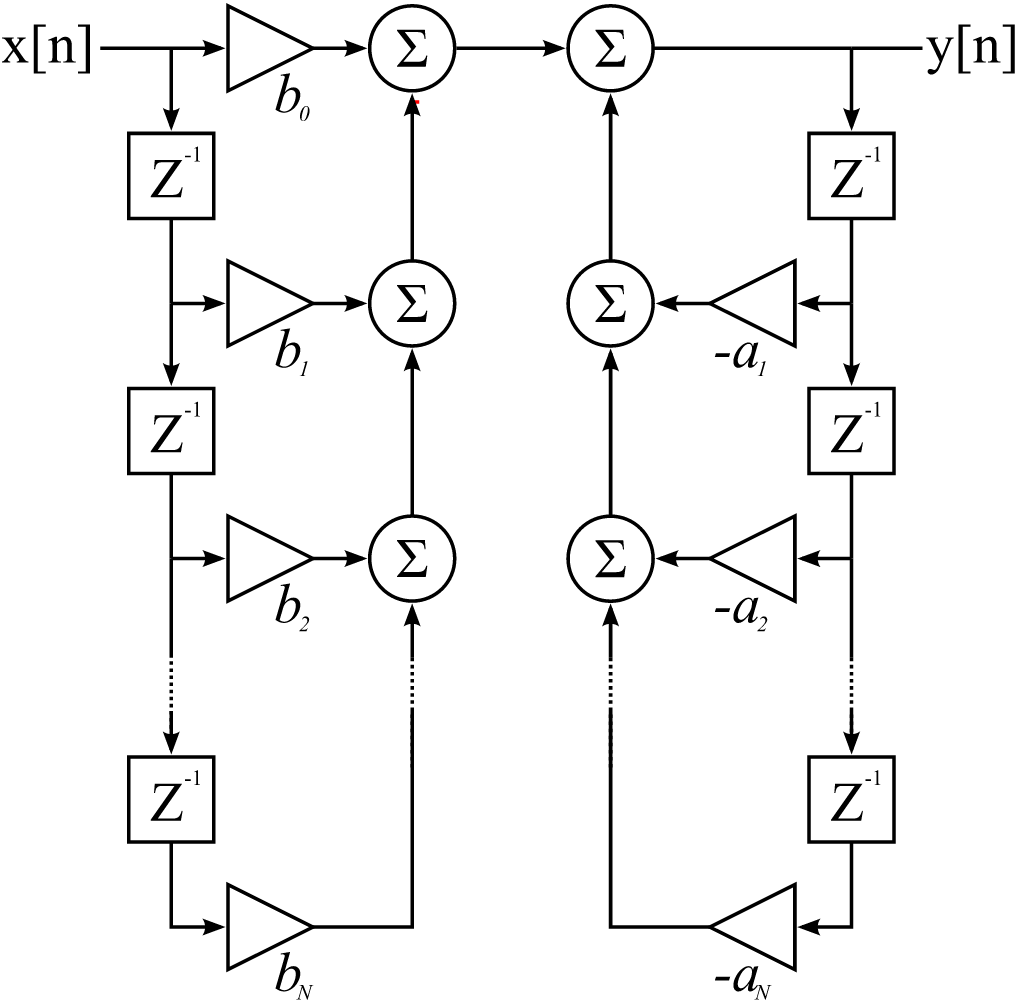
\includegraphics[scale=0.6]{IirDirectFormI.png}  
	\caption{Прямая реализация типа I БИХ фильтра}
	\label{fig:IirDirectFormI}
\end{figure}

\begin{figure}[ht]
	\centering
	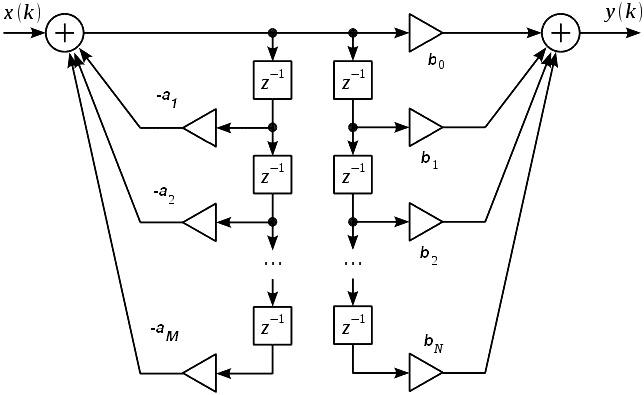
\includegraphics[scale=0.95]{IirDirectFormIINonCanonical.png}  
	\caption{Прямая реализация типа II БИХ фильтра (неканоническая)}
	\label{fig:IirDirectFormIINonCanonical}
\end{figure}

\begin{figure}[ht]
	\centering
	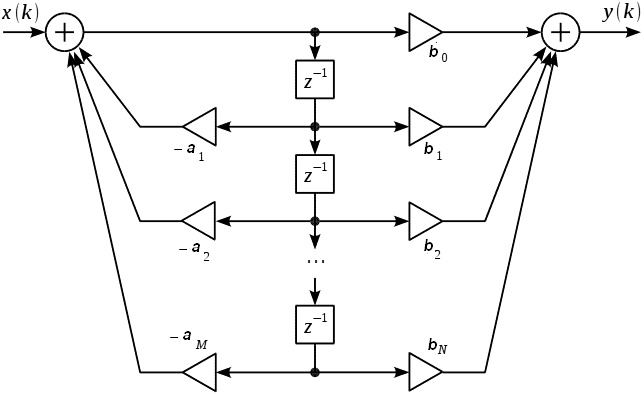
\includegraphics[scale=0.95]{IirDirectFormIICanonical.png}  
	\caption{Прямая реализация типа II БИХ фильтра (каноническая)}
	\label{fig:IirDirectFormIICanonical}
\end{figure}

В дискретных системах с постоянными параметрами соотношение между входом и выходом не зависит от порядка каскадного соединения блоков. Из этого свойства вытекает вторая прямая форма построения БИХ-фильтра. Если сначала реализовать полюсы $H(z)$ соответствующие правой части структурной схемы рисунка~\ref{fig:IirDirectFormI}, которая имеет передаточную функцию $\frac{1}{A(z)}$, а после~--- нули передаточной функцией $B(z)$, то получим структуру, показанную на рисунке~\ref{fig:IirDirectFormIINonCanonical}, которая соответствует системе уравнений~\cite{Wiki_IIR}:
\begin{gather}
	w(n) = -\sum_ {k=1}^{N} a(k)w(n - k) + x(n), \\
	y(n) = \sum_ {k=0}^{M} b(k)w(n - k).
\end{gather}

Объединив линии задержки в структуре, показанной на рисунке~\ref{fig:IirDirectFormIINonCanonical}, получим прямую каноническую форму, показанную на рисунке~\ref{fig:IirDirectFormIICanonical}~\cite{Wiki_IIR}.

В некоторых случаях, с точки зрения шумовых характеристик, фильтр, реализованный в первой прямой форме, лучше, чем в канонической~\cite{Wiki_IIR}.

% **************************************************
\subsection{Фильтр с конечной импульсной характеристикой}
\label{section:FIR}
Фильтр с конечной импульсной характеристикой (нерекурсивный фильтр, КИХ-фильтр) или FIR-фильтр (FIR сокр. от англ. \foreignlanguage{english}{finite impulse response}~--- конечная импульсная характеристика)~--- один из видов линейных цифровых фильтров, характерной особенностью которого является ограниченность по времени его импульсной характеристики (с какого-то момента времени она становится точно равной нулю). Такой фильтр называют ещё нерекурсивным из-за отсутствия обратной связи. Знаменатель передаточной функции такого фильтра~--- некая константа~\cite{Wiki_FIR}.

\subsubsection{Динамические характеристики. }
Разностное уравнение, описывающее связь между входным и выходным сигналами фильтра~\cite{Wiki_FIR}:
\begin{equation}
	y(n) = b_0 x(n) + b_1 x(n-1) +...+ b_P x(n-P),
\end{equation}
где $P$ — порядок фильтра, $x(n)$ — входной сигнал, $y(n)$ — выходной сигнал, а $b_{i}$ — коэффициенты фильтра. Иными словами, значение любого отсчёта выходного сигнала определяется суммой масштабированных значений $P$ предыдущих отсчётов. Можно сказать иначе: значение выхода фильтра в любой момент времени есть значение отклика на мгновенное значение входа и сумма всех постепенно затухающих откликов $P$ предыдущих отсчётов сигнала, которые всё ещё оказывают влияние на выход (после $P$-отсчётов импульсная переходная функция становится равной нулю, как уже было сказано, поэтому все члены после $P$-го тоже станут равными нулю). Запишем предыдущее уравнение в более ёмком виде:
\begin{equation}
	y(n) = \sum_{i=0}^{P} b_i x(n-i).
\end{equation}
Для того, чтобы найти ядро фильтра, положим:
\begin{equation}
	x(n) = \delta(n),
\end{equation}
\begin{explanation}
	где &$\delta(n)$& дельта-функция.
\end{explanation}
Тогда импульсная характеристика КИХ-фильтра может быть записана как:
\begin{equation}
	h(n) = \sum_{i=0}^{P}b_i \delta(n-i).
\end{equation}
Z-преобразование импульсной характеристики даёт нам передаточную функцию КИХ-фильтра~\cite{Wiki_FIR}:
\begin{equation}
	H(z) = \sum_{i=0}^{P}b_i z^{-i}.
\end{equation}

\subsubsection{Свойства. }
КИХ-фильтр обладает рядом полезных свойств, из-за которых он иногда более предпочтителен в использовании, чем БИХ-фильтр. Вот некоторые из них~\cite{Wiki_FIR}:
\begin{itemize}
	\item КИХ-фильтры устойчивы;
	\item КИХ-фильтры при реализации не требуют наличия обратной связи;
	\item Фаза КИХ-фильтров может быть сделана линейной.
\end{itemize}

\subsubsection{Прямая форма КИХ-фильтра. }
КИХ-фильтры могут быть реализованы с использованием трёх элементов: умножитель, сумматор и блок задержки. Вариант, показанный на рисунке~\ref{fig:FirStructure}, есть прямая реализация КИХ-фильтров типа I~\cite{Wiki_FIR}.

\begin{figure}[ht]
	\centering
	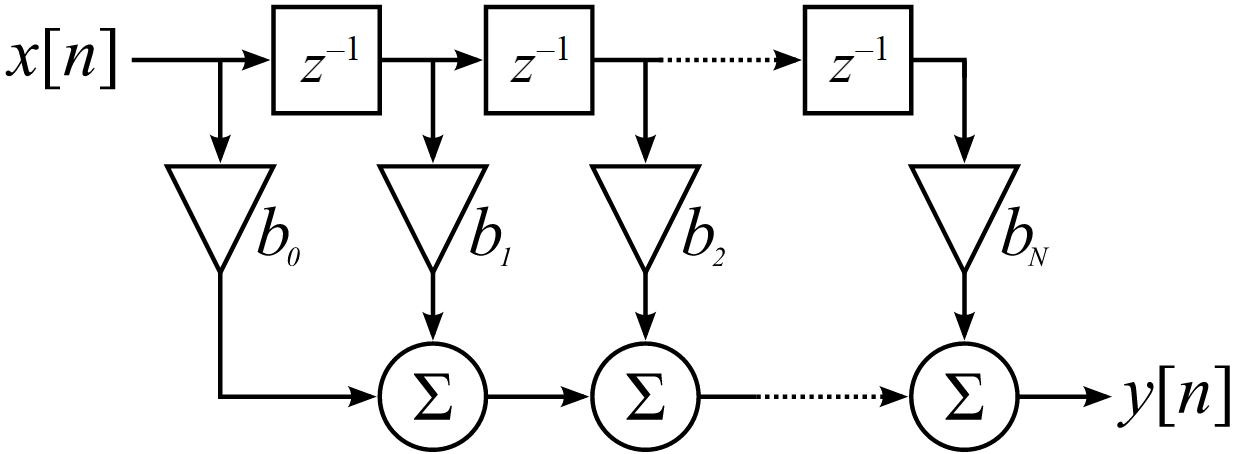
\includegraphics[scale=0.45]{FirStructure.png}  
	\caption{Реализация прямой формы КИХ-фильтра}
	\label{fig:FirStructure}
\end{figure}